\chapter{PROCEDIMENTOS METODOLÓGICOS}
\label{chap:metodologia}



%Procedimentos Metodológicos relaciona-se ao passo-a-passo da execução do trabalho pesquisa: como se obterá os dados necessários para respondem à sua questão de pesquisa? Um bom ponto de partida para escrever os procedimentos é detalhar extensamente cada objetivo específico.

%Para que os resultados encontrados sejam considerados válidos, é preciso respeitar e seguir as tradições de cada área de pesquisa. As estratégias de levantamento de dados, e de registro e análise do material coletado, mudam conforme a natureza da pesquisa. Seguem alguns exemplos:


A metodologia do trabalho adotou revisão sistemática da literatura \cite{kitchenham} como estratégia de pesquisa. Os trabalhos e dados relacionados aos fatores que influenciam a comunicação de requisitos na engenharia de software foram coletados. Para alcançar tal objetivo os passos ilustrados na Figura \ref{fig:metodologia} foram executados.

\begin{figure}[h!]
	\caption{Metodologia da pesquisa.}
	\begin{center}
	    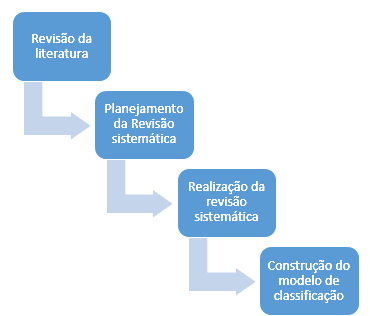
\includegraphics[scale=1.0]{figuras/metodologia}
	\end{center}
	\label{fig:metodologia}
	\legend{Fonte: Autor.}
\end{figure}
   
   
\section{Revisão da literatura}

    Como o objetivo deste trabalho foi identificar fatores de comunicação, em primeiro momento foi realizado uma revisão da literatura que consiste em uma pesquisa bibliográfica em trabalhos com conceitos em comum ou relacionados. Os estudos mais próximos com os objetivos desse trabalho foram descritos no Capítulo \ref{sec:objetivo-geral-2}. %resultando em um conjunto de trabalhos que serão posteriormente utilizados nos passos descritos nas seguintes seções. 
     
\section{Planejamento da Revisão Sistemática}

    Para a realização de revisões sistemática da literatura, foi necessário definir um protocolo de pesquisa. O protocolo da revisão seguido neste trabalho é descrito com detalhes na Seção \ref{sec:protocolo}.
    
    O protocolo foi desenvolvido seguindo as \emph{guidelines} de \cite{kitchenham}, explicadas na Seção \ref{sec:fund_slr}. A definição e execução da revisão sistemática foram suportadas pela ferramenta Parsifal \footnote{https://parsif.al/}. 
     
 \section{Realização da revisão Sistemática}  
 O protocolo definido foi seguido para obter estudos relacionados a comunicação de requisitos no processo de desenvolvimento de software. Esses estudos constituíram a fonte de dados para a obtenção dos fatores que influenciam a comunicação de requisitos.
 
    
%\subsection{Classificação dos fatores}

\section{Construção do modelo de classificação}

A partir dos fatores selecionados nos estudos provenientes da revisão sistemática, foi realizado então uma análise individual para identificar se a ocorrência do mesmo auxilia ou piora a comunicação. 

Com base no processo de comunicação (ver Figura \ref{fig:processocomunicacao}), foi identificado em qual ponto do processo cada fator obtido na revisão sistemática atua. Sabendo que no processo de comunicação envolvem os conceitos descritos na Seção \ref{sec:fund_comunicacao} (Codificação da informação, Decodificação da informação, Emissor, Receptor, Canal de comunicação, Mensagem e \emph{Feedback}), foi criado um modelo de classificação desses fatores. %Cada  para cada fa com "Seções" positivo, negativo.

%\begin{itemize}
%    \item Codificação da informação
%    \item Decodificação da informação
%    \item Emissor
%    \item Receptor 
%    \item Canal de comunicação 
%    \item Mensagem 
%    \item Feedback
%\end{itemize}



O modelo demonstra onde o fator atua no processo de comunicação e qual o impacto do mesmo, sendo este positivo ou negativo. Além disso, conceitos como os listados abaixo estão inclusos no modelo:

\begin{itemize} 
 \item Positivos: 
    \begin{itemize} 
        \item Melhoria 
        \item Boas práticas
    \end{itemize}

 \item Negativos: 
    \begin{itemize}
        \item Ruídos de comunicação
        \item Empecilhos e impedimentos 
    \end{itemize}
\end{itemize}

Como resultado foi proposto um modelo que demonstra onde os fatores atuam no processo de comunicação.


\begin{comment}
\section{Validação do modelo}
A validação do modelo ainda será planejada com detalhes, porém espera-se obter \emph{feedback} de profissionais e \emph{experts} em desenvolvimento de software da academia seguindo o modelo de transferência de tecnologia proposto por \cite{gorschekTechnology}. A validação será baseada em métodos e diretrizes de engenharia de software empírica \cite{wieringa} \cite{carolynqualitative}. Para conduzir a investigação com os profissionais, priorizar-se-á por aplicar uma abordagem de pesquisa qualitativa adotando entrevistas semiestruturadas como estratégia para alcançar os objetivos do estudo \cite{merriamqualitative}.
\end{comment}


%We followed the guidelines proposed by Runeson and Martin \cite{runeson} to investigate a contemporary phenomenon, i.e. the application of Uni-REPM SCS, within its real-life context (maturity evaluation of the companies). There are five major process steps to go through in the case study research process \cite{runeson} as presented in Figure \ref{fig:casestudysteps}.

\begin{comment}
\section{Cronograma de Execução}

Nesta seção será apresentado o cronograma de execução deste trabalho, ilustrado na seguinte tabela: 


\begin{table}[h!]
\centering
\resizebox{\textwidth}{!}{\begin{tabular}{|l|c|c|c|c|c|c|c|c|c|c|c|c|c|c|}
\hline
\multicolumn{1}{|c|}{\multirow{2}{*}{ATIVIDADES}} & \multicolumn{14}{c|}{2018} \\ \cline{2-15} 
\multicolumn{1}{|c|}{} & \multicolumn{2}{c|}{Mai} & \multicolumn{2}{c|}{Jun} & \multicolumn{2}{c|}{Jul} & \multicolumn{2}{c|}{Ago} & \multicolumn{2}{c|}{Set} & \multicolumn{2}{c|}{Out} & \multicolumn{2}{c|}{Nov} \\ \hline
\begin{tabular}[c]{@{}l@{}}
%Estudo de Domínio & x & x & x &  &  &  &  &  &  &  &  &  &  & - \\ \hline

Elaboração do protocolo da revisão sistemática\end{tabular} & x & x & x &  &  &  &  &  &  &  &  &  &  &  \\ \hline

Defesa do projeto &  &  &  & x &  &  &  &  &  &  &  &  &  &  \\ \hline

Condução da revisão sistemática &  &  &  &  & x & x & x & x &  &  &  &  &  &  \\ \hline

Construção do modelo &  &  &  &  &  &  &  & x &x  &x  &  &  &  &  \\ \hline

Validação do modelo &  &  &  &  &  &  &  &  &  &  & x & x &  &  \\ \hline

Análise dos resultados &  &  &  &  &  &  &  &  &  &  &x  &x  &x  &  \\ \hline

Escrita da monografia &  &  &  &  &  &  &  &  &  &  &  & x & x &  \\ \hline

Defesa do Trabalho Final &  &  &  &  &  &  &  &  &  &  &  &  &  & x \\ \hline
\end{tabular}}
\end{table}

No próximo capítulo é descrito o protocolo da revisão sistemática que será utilizado neste trabalho.
\end{comment}

